#
# Copyright 2006-2017 Vladimir Veshnev, Aleksey Geraskin, Marina Nurlygayanova,
# Timur Nurlygayanov
#
# This file is part of MD program.
#
# MD is free software : you can redistribute it and / or modify
# it under the terms of the GNU General Public License as published by
# the Free Software Foundation, either version 3 of the License, or
# (at your option) any later version.
# 
# MD is distributed in the hope that it will be useful,
# but WITHOUT ANY WARRANTY; without even the implied warranty of
# MERCHANTABILITY or FITNESS FOR A PARTICULAR PURPOSE.See the
# GNU General Public License for more details.
#
# You should have received a copy of the GNU General Public License
# along with MD. If not, see <http://www.gnu.org/licenses/>
#

\documentclass[a4paper]{article}

\usepackage{color}
\usepackage[russian,english]{babel}
\usepackage[T1]{fontenc}
\usepackage[utf8]{inputenc}
\usepackage{amsmath,amssymb}
\usepackage{mathtext}
\usepackage{graphicx}
\usepackage[T1]{fontenc}
\usepackage[normalem]{ulem}
\usepackage[nottoc,numbib]{tocbibind}
\usepackage{fullpage}
\usepackage[pdftex]{lscape}

\usepackage{listings}
\lstset{language=C++,inputencoding=cp1251}

\ULdepth = 0.16em

\begin{document}

\selectlanguage{russian}

\tableofcontents
\pagebreak

\section{Введение}

Данная статья посвящена рассмотрению алгоритма моделирования системы идеальных твёрдых сфер вблизи идеальных стенок для компьютерных экспериментов по изучению процесса кристаллизации жидкости твёрдых сфер вблизи идеальной стенки. В этой статье описывается модель жёстких сфер, модель идеальной стенки и модель используемых периодических граничных условий.

Используемый нами ранее алгоритм \cite{Veshnev_Nurlygayanov_Cristalization_of_hard_spheres_near_the_hard_wall_ru_2011} был существенно переработан, в частности, был применён ряд оптимизаций \cite{Miller_Luding_Event_driven_molecular_dynamics_in_parallel} \cite{Rapaport_The_Event_Driven_Approach_to_N_Body_Simulation} \cite{Belkin_MMD_2006}.

Описание, приведённое в данной статье, соответствует программе, написанной для моделирования исследуемой нами системы жёстких сфер, и может быть использовано для анализа алгоритма, реализованного в написанной программе.

Программа, реализующая описанный в этой статье алгоритм, написана на языке С++. Существует несколько версий программы, в которых реализация периодических граничных условий и некоторых функций может отличаться от описанного в этой статье алгоритма, в данной статье описывается только последний вариант реализации алгоритма, актуальный на данный момент, а так же приводится краткий обзор используемых ранее алгоритмов и периодических граничных условий с целью исторического обзора пути развития применяемых нами алгоритмов, а так же в целях объяснения причин, по которым мы выбрали именно данные граничные условия и определённую реализацию некоторых алгоритмов (выбор используемых алгоритмов, в основном, продиктован их оптимальностью - предпочтение отдавалось алгоритмам, требующим наименьшего времени для получения точного решения).

В разработке физической модели моделируемой системы и алгоритма, описанного в данной статье и реализованного в программе на языке С++, принимали активное участие:

Вешнев Владимир Петрович

Гераськин Алексей Сергеевич

Нурлыгаянова Марина Николаевна

Нурлыгаянов Тимур Артурович

Данная статья и любая информация, описанная в ней, а так же исходный код программы, реализующий данный алгоритм, может быть использован, изменён или опубликован только с согласия всех описанных лиц.

Во время работы над этой статьёй авторы использовали различную литературу, ссылки на которую будут даны в тексте статьи.

\newpage
\section{Общее описание моделируемой системы}

\subsection{Модель идеальной стенки}
Модель идеальной жёсткой стенки используется для симуляции границы системы, через которую частицы не могут покинуть рассматриваемый объём. Модель идеальной жёсткой стенки широко применяется в различных компьютерных экспериментах и теоретических исследованиях.

Идеальная жёсткая стенка имеет следующие свойства:

 - Имеет большую массу, стремящуюся к бесконечности:
 
\begin{equation}
        M_{ideal \; wall} \to \infty,
\end{equation}

 - Является абсолютно гладкой для всех частиц в системе, т.е. при касании стенки любой частицей в системе возникающая между этой частицей и идеальной стенкой сила трения равна нулю,
 
 - Является атермичной, т.е. не изменяет кинетическую энергию частиц в системе,
 
 - Имеет импульс, равный нулю, т.е. не движется:
 
\begin{equation}
        p_{ideal \; wall} = 0,
\end{equation}


\subsection{Модель идеальной жёсткой сферы}
В данном эксперименте мы используем модель идеальной жёсткой сферы для моделирования частиц. Эта модель применяется во многих компьютерных экспериментах \cite{Rosenbluth_Chem_Phys_22_881_1954} \cite{Wood_and_Jacobson_1957} \cite{Alder_and_Wainwright_Phase_Transition_for_a_Hard_Sphere_System}.

Идеальная жёсткая сфера обладает следующими свойствами:

 - Имеет форму идеального равномерного шара, центр масс которого находится в его геометрическом центре \cite{Dzonkali_1989_Physics_T1},
     
 - Не совершает вращательного движения, 
 
 - Является абсолютно гладкой для других идеальных жёстких сфер и идеальной стенки (т.е. при соприкосновении с другими жёсткими сферами или идеальной стенкой сила трения $ F_{тр} $, возникающая между двумя идеальными жёсткими сферами или идеальной жёсткой сферой и идеальной стенкой, равна нулю),
 
 - Сталкивается с другими идеальными жёсткими сферами или идеальной стенкой мгновенно, т.е. промежуток времени $ \Delta t $, на протяжении которого происходит соударение, стремится к нулю,
 
 - В любой момент времени, если идеальная жёсткая сфера не сталкивается с другой идеальной жёсткой сферой или с идеальной стенкой, эта идеальная жёсткая сфера движется равномерно и прямолинейно, 
 
 - Имеет ненулевой размер и занимает объём системы, равный $ \frac{4}{3} \pi R^3 $, где $ R $ - радиус идеальной сферы. 
 
 - Сталкивается с другими идеальными жёсткими сферами и идеальной стенкой абсолютно упруго. Потенциал взаимодействия между двумя идеальными жёсткими сферами описывается следующей системой уравнений:

\begin{equation}\label{eq:rule_of_potential_between_two_particles}
    \begin{cases}
        p = 0, r > 2R,
        \\
        p = \infty, r <= 2R,
    \end{cases}
\end{equation}
где $ p $ - потенциал взаимодействия между двумя идеальными сферами, $ R $ - радиус идеальной жёсткой сферы, $ r $ - расстояние между центрами  идеальных жёстких сфер. 

Потенциал взаимодействия идеальной жёсткой сферы с идеальными стенками, которые ограничивают рассматриваемую нами систему, можно описать системой уравнений

\begin{equation}\label{eq:rule_of_potential_between_particles_and_walls}
    \begin{cases}
        p = 0, r > R,
        \\
        p = \infty, r <= R,
    \end{cases}
\end{equation}
где $ p $ - потенциал взаимодействия между идеальной жёсткой сферой и идеальной твёрдой стенкой, $ R $ - радиус идеальной жёсткой сферы, $ r $ - расстояние между центром идеальной жёсткой сферы и идеальной твёрдой стенкой.

Потенциал взаимодействия между двумя жёсткими сферами или идеальной стенкой и жёсткой сферой, равный $ \infty $, накладывает условие невозможности такого состояния системы, в котором расстояние между центрами двух идеальных жёстких сфер было бы меньше $ 2R $, а расстояние центра идеальной жёсткой сферы и идеальной стенкой было бы меньше $ R $.

Идеальная жёсткая сфера соударяется с идеальной стенкой абсолютно упруго, при этом энергия частицы не изменяется, изменяется лишь проекция скорости частицы на ось $ OX $:

\begin{equation}
    v'_x = -v_x,
\end{equation}
где $ v_x $ - проекция скорости частицы на ось $ OX $ до соударения с идеальной стенкой, $ v'_x $ - проекция скорости частицы на ось $ OX $ после соударения с идеальной стенкой.

Условие соударения идеальной жёсткой сферы с идеальными стенками в рассматриваемой системе можно записать так:

\begin{equation}\label{eq:condition_of_collision_with_ideal_wall}
    \begin{cases}
        x = R, v_x < 0.0
        \\
        or
        \\
        x = L - R, v_x > 0.0,
    \end{cases}
\end{equation}
где $ x $ - это значение координаты частицы вдоль оси $ OX $, $ v_x $ - значение проекции скорости частицы на ось $ OX $, $ R $ - радиус идеальной сферы, $ L $ - расстояние между двумя идеальными стенками в системе.

Частицы не могут находиться на расстоянии менее R от идеальной стенки и координаты всех частиц в системе в любой момент времени удовлетворяют следующим правилам:

\begin{equation}\label{eq:particles_and_ideal_wall}
    \begin{cases}
        x >= R
        \\
        x <= L - R.
    \end{cases}
\end{equation}


\subsection{Периодические граничные условия}

Периодические граничные условия не дают частицам беспрепятственно покидать выделенный объём, позволяя тем самым моделировать бесконечную систему частиц, рассчитывая динамику системы, содержащую только небольшое количество частиц.

Условия, которые накладываются на частицы, находящиеся в моделируемой системе:

1. Центр каждой частицы всегда находится в системе или на её границе. Положения центров каждой частицы в системе в любой момент времени удовлетворяют следующей системе уравнений:

\begin{equation}
    \begin{cases}
        x >= R,
        \\
        x <= L - R,
        \\
        0 <= y <= A,
        \\
        0 <= z <= A,
    \end{cases}
\end{equation}
где $ x $, $ y $ и $ z $ - координаты частицы в трехмерной системе координат, R - радиус частицы, представляющей из себя идеальную жесткую сферу, L - расстояние между двумя идеальными стенками и A - это расстояние между двумя противоположными плоскостями, представляющими периодические границы.

2. Частицы могут пересекать границы системы, заданные уравнениями:

\begin{equation}
y = 0
\end{equation}
\begin{equation}
y = A
\end{equation}
\begin{equation}
z = 0
\end{equation}
\begin{equation}
z = A
\end{equation}

И не могут пересекать границы, заданные уравнением:

\begin{equation}
x = 0
\end{equation}
\begin{equation}
x = L
\end{equation}

т.к. эти границы являются идеальными стенками. 

При пересечении границы в момент пересечения одной из периодических границ системы центром частицы на одной из других периодических границ создаётся частица с энергией, равной энергии данной частицы и движущаяся согласно тому же уравнению движения, что и исходная частица. Исходная частица, пересекающая границу системы, при этом удаляется.

3. Если для координат центра частицы выполняется одно из следующих условий:

\begin{equation}
0 <= y <= 1
\end{equation}
\begin{equation}
A - 1 <= y <= A
\end{equation}
\begin{equation}
0 <= z <= 1
\end{equation}
\begin{equation}
A - 1 <= z <= A
\end{equation}
то существует один "образ" данной частицы, который движется согласно тому же уравнению движения, что и исходная частица. При пересечении центром частицы одной из границ системы "образ" становится обычной частицей, а сама частица уничтожается. При этом энергия частицы не изменяется, меняются лишь координаты центра частицы.

4. Центр "образа" всегда находится вне системы, что позволяет не учитывать "образ" как отдельную частицу. Любой частице в системе может соответствовать либо ни одного "образа", либо только один "образ".

5. При столкновении частицы или ее "образа" с другой частицей, "образом" другой частицей или идеальной стенкой скорость частицы изменяется, как и её уравнение движения. При этом "образ", соответствующий этой частице, уничтожается (если он существовал) и создаётся новый "образ" (если это необходимо - см. пункт №3), который будет двигаться согласно новому уравнению движения.

6. "Образ" может иметь скорость, отличную от скорости самой частицы, при этом он обязательно должен перемещаться согласно тому же уравнению движения, что и исходная частица (по той же линии скорости или по линии скорости, полученной параллельным переносом по OX, что будет рассмотрено отдельно). При столкновении "образа" с другой частицей или "образом" другой частицы учитывается скорость исходной частицы, а не её "образа" (при расчёте новых скоростей), что позволяет сохранять общую энергию системы постоянной.

7. При создании "образа" некоторой частицы позиция его центра выбирается так, чтобы он находился на линии скорости исходной частицы, в точке, из которой он достигнет одной из периодических границ системы в то же самое время, когда центр исходной частицы будет находиться в плоскости пересекаемой ею границы.

Рассмотрим подробнее вычисление координат центра создаваемого "образа". Уравнение движения центра сферы по прямолинейной траектории с постоянной скоростью в векторном виде можно записать так:

\begin{equation}
\vec{r} = \vec{r}_0 + \vec{v}*t
\end{equation}

где $ \vec{r} $ - радиус вектор нового положения центра частицы, $ \vec{r}_0 $ - радиус вектор начального положения центра частицы, $ \vec{v} $ - скорость частицы и $ t $ - время движения.

Распишем это выражение в проекциях на оси координат:

\begin{equation}\label{eq:r_scalar}
    \begin{cases}
        r_x = r_{0x} + v_x * t,
        \\
        r_y = r_{0y} + v_y * t,
        \\
        r_z = r_{0z} + v_z * t.
    \end{cases}
\end{equation}

из этой системы уравнений получаем:

\begin{equation}\label{eq:t_simple}
    \begin{cases}
        t = \displaystyle\frac{r_x - r_{0x}}{v_x},
        \\
        t = \displaystyle\frac{r_y - r_{0y}}{v_y},
        \\
        t = \displaystyle\frac{r_z - r_{0z}}{v_z}.
    \end{cases}
\end{equation}

Полученная система уравнений (\ref{eq:t_simple}) позволяет рассчитывать время, требующееся для перемещения центра частицы из одной позиции в другую.

Когда центр частицы находится на границе системы, прямая, описывающая уравнение её движения, пересекает плоскость, которой описана эта граница. Рассчитав времена, которые потребуются частице для того, чтобы её центр оказался в плоскости каждой границы, мы можем вычислить границу, на которой центр выбранной частицы окажется быстрее всего. Для этого необходимо решить четыре системы уравнений (одна система уравнений для каждой периодической границы):

\begin{equation}
    \begin{cases}
        y = 0,
        \\
        t = \displaystyle\frac{r_y - r_{0y}}{v_y}.
    \end{cases}
\end{equation}

\begin{equation}
    \begin{cases}
        y = A,
        \\
        t = \displaystyle\frac{r_y - r_{0y}}{v_y}.
    \end{cases}
\end{equation}

\begin{equation}
    \begin{cases}
        z = 0,
        \\
        t = \displaystyle\frac{r_z - r_{0z}}{v_z}.
    \end{cases}
\end{equation}

\begin{equation}
    \begin{cases}
        z = A,
        \\
        t = \displaystyle\frac{r_z - r_{0z}}{v_z}.
    \end{cases}
\end{equation}

полагая при решении этих систем уравнений $ r_y = y $ и $ r_z = z $, мы получим 4 решения для  $t$:

\begin{equation}\label{eq:t_end}
    \begin{cases}
        t_1 = \displaystyle\frac{0 - r_{0y}}{v_y},
        \\
        t_2 = \displaystyle\frac{A - r_{0y}}{v_y},
        \\
        t_3 = \displaystyle\frac{0 - r_{0z}}{v_z},
        \\
        t_4 = \displaystyle\frac{A - r_{0z}}{v_z}.
    \end{cases}
\end{equation}
где $ r_{0y} $, $ r_{0z} $ - проекции радиус вектора текущего положения частицы на оси $ OY $ и $ OZ $.

Необходимо найти $ t_{min} $, удовлетворяющее условиям:

\begin{equation}\label{eq:t_min}
    \begin{cases}
        t_{min} > 0,
        \\
        t_{min} <= t_1,
        \\
        t_{min} <= t_2,
        \\
        t_{min} <= t_3,
        \\
        t_{min} <= t_4,
    \end{cases}
\end{equation}
где $ t_{min} $ есть время, за которое частица достигнет ближайшей границы системы, если будет двигаться с текущей скоростью. В соответствии с условием №7 'образ', соответствующий данной частице, должен  за это же время достигнуть другой периодической границы системы.

Для того, чтобы вычислить координаты центра создаваемого "образа", возьмём новые значения $ v_x $, $ v_y $ и $ v_z $, равные:

\begin{equation}
    \begin{cases}
        v'_x = - v_x,
        \\
        v'_y = - v_y,
        \\
        v'_z = -v_z.
    \end{cases}
\end{equation}

и рассчитаем для них уравнения (\ref{eq:t_end}) и (\ref{eq:t_min}), подставив полученное в результате решения этих уравнений значение $ t'_{min} $  значения $ v'_x $, $ v'_y $ и $ v'_z $ в систему уравнений (\ref{eq:r_scalar}), получим:

\begin{equation}
    \begin{cases}
        r'_x = r_{0x} + v'_x * t'_{min},
        \\
        r'_y = r_{0y} + v'_y * t'_{min},
        \\
        r'_z = r_{0z} + v'_z * t'_{min}.
    \end{cases}
\end{equation}
где $ r'_x $, $ r'_y $ и $ r'_z $ есть значения новых координат центра частицы, которые она будет иметь после прохождения через периодическую границу.

Сложив $ t_{min} $ и $ t'_{min} $ и подставив получившееся значение $ t $ в систему уравнений (\ref{eq:r_scalar}) мы получим значения координат создаваемого образа, соответствующего данной частице:

\begin{equation}
    \begin{cases}
        r''_x = r_{0x} + v'_x * (t_{min} + t'_{min}),
        \\
        r''_y = r_{0y} + v'_y * (t_{min} + t'_{min}),
        \\
        r''_z = r_{0z} + v'_z * (t_{min} + t'_{min}).
    \end{cases}
\end{equation}
здесь $ r''_x $, $ r''_y $ и $ r''_z $ - координаты создаваемого образа, $ r_{0x} $, $ r_{0y} $ и $ r_{0z} $ - текущие координаты исходной частицы, для которой необходимо создать виртуальную частицу.


\newpage
\section{Расчёт столкновения идеальных жёстких сфер}
Необходимо описать подробно.
\subsection{Расчёт времени до соударения двух идеальных жёстких сфер}
Необходимо описать подробно.

\subsection{Расчёт новых скоростей идеальных жёстких сфер после соударения}
Рассмотрим общий случай соударения двух частиц, представляющих из себя идеальные жёсткие сферы.

При любом столкновении двух идеальных жёстких сфер центры масс этих сфер, а так же точка соприкосновения поверхностей этих двух сфер лежат в одной плоскости.

Рассмотрим проекцию двух сфер и их скоростей на эту плоскость в момент соударения. 

\begin{center}
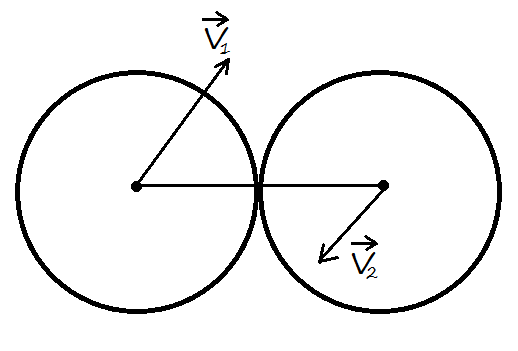
\includegraphics[scale=0.3]{collission_of_two_particles.png}
\end{center}

Здесь $ \vec{v}_1 $ - скорость первой частицы, $ \vec{v}_2 $ - скорость второй частицы.

Так как рассматриваемые сферы являются равномерными идеальными сферами и точка касания двух сфер находится на одной линии с центрами масс обеих сфер, то и силы, действующие со стороны первой частицы на вторую и со стороны второй частицы на первую будут направлены по линии, соединяющей центры масс сфер.

Идеальные сферы являются абсолютно гладкими и не могут совершать вращательное движение, поэтому силы, действующие на первую и вторую частицы, действуют только вдоль линии, соединяющей центры масс данных частиц.

Изобразим действующие на обе идеальные сферы силы:


Согласно третьему закону Ньютона должно выполняться равенство:

\begin{equation}\label{eq:Neuton_rule2}
        \vec{F}_1 = - \vec{F}_2
\end{equation}

Распишем скорость $ \vec{v}_1 $ как сумму $ \vec{v}_{1\perp} $ и $ \vec{v}_{1\parallel} $ и скорость $ \vec{v}_2 $ как сумму $ \vec{v}_{2\perp} $ и $ \vec{v}_{2\parallel} $, где $ \vec{v}_{1\perp} $ и $ \vec{v}_{2\perp} $ составляющие скоростей $ \vec{v}_1 $ и $ \vec{v}_2 $, перпендикулярные линии, соединяющей центры сталкивающихся частиц, $ \vec{v}_{1\parallel} $ и $ \vec{v}_{2\parallel} $ - параллельные составляющие скоростей $ \vec{v}_1 $ и $ \vec{v}_2 $ относительно линии, соединяющей центры частиц.

Учитывая, что силы, действующие на первую и вторую частицы в момент их соударения, действуют только вдоль прямой, соединяющей центры масс данных частиц, можно утверждать, что составляющие скоростей движения частиц, перпендикулярные линии, соединяющей центры этих частиц, не влияют на величину и направление сил $ \vec{F}_1 $ и $ \vec{F}_2 $.

Поэтому учитывая, что масса идеальных жёстких сфер постоянна, мы можем записать:

\begin{equation}\label{eq:velocities_and_forces_for_two_particles}
    \begin{cases}
        \vec{F}_1 = \displaystyle\frac{m_1*d\vec{v}_{1\parallel}}{dt},
        \\
        \\
        \displaystyle\frac{m_1*d\vec{v}_{1\perp}}{dt} = 0,
        \\
        \\
        \vec{F}_2 = \displaystyle\frac{m_2*d\vec{v}_{2\parallel}}{dt},
        \\
        \\
        \displaystyle\frac{m_2*d\vec{v}_{2\perp}}{dt} = 0,
    \end{cases}
\end{equation}

Учитывая второй закон Ньютона для данной системы двух идеальных твёрдых сфер (\ref{eq:Neuton_rule2}), а так же то, что массы всех идеальных твёрдых сфер равны, мы можем записать (\ref{eq:velocities_and_forces_for_two_particles}) в виде:

\begin{equation}\label{eq:velocities_and_forces_for_two_particles2}
    \begin{cases}
        \displaystyle\frac{d\vec{v}_{2\parallel}}{dt} = -\displaystyle\frac{d\vec{v}_{1\parallel}}{dt},
        \\
        \\
        \vec{v}_{1\perp} = const,
        \\
        \\
        \vec{v}_{2\perp} = const,
    \end{cases}
\end{equation}

Идеальные жёсткие сферы соударяются абсолютно упруго, а значит при соударении двух идеальных жёстких сфер должны выполняться закон сохранения импульса и закон сохранения энергии.

Закон сохранения импульса для рассматриваемой системы двух частиц  может быть записан как

\begin{equation}\label{eq:rule_of_contant_impulse}
    \begin{cases}
        \vec{v}_{1\perp} + \vec{v}_{2\perp} = \vec{v}\ '_{1\perp} + \vec{v}\ '_{2\perp},
        \\
        \vec{v}_{1\parallel} + \vec{v}_{2\parallel} = \vec{v}\ '_{1\parallel} + \vec{v}\ '_{2\parallel},
    \end{cases}
\end{equation}
где $ \vec{v}\ '_{1\perp} $, $ \vec{v}\ '_{1\parallel} $, $ \vec{v}\ '_{2\perp} $, $ \vec{v}\ '_{2\parallel} $ - скорости частиц после соударения.

Запишем закон сохранения энергии для данной системы из двух сталкивающихся идеальных сфер:

\begin{equation}\label{eq:rule_of_contant_energy}
    \begin{cases}
        E_1 = \displaystyle\frac{mv^2_{1\perp}}{2} + \displaystyle\frac{mv^2_{1\parallel}}{2} + \displaystyle\frac{mv^2_{2\perp}}{2} + \displaystyle\frac{mv^2_{2\parallel}}{2},
        \\
        \\
        E_2 = \displaystyle\frac{mv\ '^2_{1\perp}}{2} + \displaystyle\frac{mv\ '^2_{1\parallel}}{2} + \displaystyle\frac{mv\ '^2_{2\perp}}{2} + \displaystyle\frac{mv\ '^2_{2\parallel}}{2},
        \\
        \\
        E_1 = E_2,
    \end{cases}
\end{equation}
где $ E_1 $ - полная кинетическая энергия системы из двух частиц перед соударением, $ E_2 $ - полная кинетическая энергия системы из двух частиц после соударения. Потенциальная энергия частиц при соударении не изменяется, т.к. происходит абсолютно упругий удар.

Учитывая (\ref{eq:velocities_and_forces_for_two_particles2}) мы можем записать, что $ \vec{v}_{1\perp} = \vec{v}\ '_{1\perp} $ и $ \vec{v}_{2\perp} = \vec{v}\ '_{2\perp} $, тогда учитывая закон сохранения импульса (\ref{eq:rule_of_contant_impulse}) и закон сохранения энергии (\ref{eq:rule_of_contant_energy}) мы можем записать следующую систему уравнений:

\begin{equation}
    \begin{cases}
        \vec{v}_{1\parallel} + \vec{v}_{2\parallel} = \vec{v}\ '_{1\parallel} + \vec{v}\ '_{2\parallel},
        \\
        \displaystyle\frac{mv^2_{1\parallel}}{2} + \displaystyle\frac{mv^2_{2\parallel}}{2} = \displaystyle\frac{mv\ '^2_{1\parallel}}{2} + \displaystyle\frac{mv\ '^2_{2\parallel}}{2}
    \end{cases}
\end{equation}

Сразу упростим второе уравнение, учтя равенство масс двух идеальных жёстких сфер:

\begin{equation}\label{eq:start_of_system_for_new_speed}
    \begin{cases}
        \vec{v}_{1\parallel} + \vec{v}_{2\parallel} = \vec{v}\ '_{1\parallel} + \vec{v}\ '_{2\parallel},
        \\
        v^2_{1\parallel} + v^2_{2\parallel} = v\ '^2_{1\parallel} + v\ '^2_{2\parallel}
    \end{cases}
\end{equation}

Преобразуем первое уравнение в (\ref{eq:start_of_system_for_new_speed}), домножив обе части уравнения на $ \vec{v}_{1\parallel} $:

\begin{equation}
    \vec{v}^2_{1\parallel} + \vec{v}_{2\parallel}\vec{v}_{1\parallel} = \vec{v}\ '_{1\parallel}\vec{v}_{1\parallel} + \vec{v}\ '_{2\parallel}\vec{v}_{1\parallel}
\end{equation}
Теперь выразим из этого уравнения $ \vec{v}^2_{1\parallel} $ и подставим получившееся выражение во второе уравнение системы уравнений (\ref{eq:start_of_system_for_new_speed}), получим:

\begin{equation}
    \vec{v}_{1\parallel}(\vec{v}\ '_{1\parallel} + \vec{v}\ '_{2\parallel} - \vec{v}_{2\parallel}) + \vec{v}^2_{2\parallel} = \vec{v}\ '^2_{1\parallel} + \vec{v}\ '^2_{2\parallel}
\end{equation}

и выразим из полученного уравнения $ \vec{v}_{1\parallel} $:

\begin{equation}
    \vec{v}_{1\parallel} = \frac{\vec{v}\ '^2_{1\parallel} + \vec{v}\ '^2_{2\parallel} - \vec{v}^2_{2\parallel}}{\vec{v}\ '_{1\parallel} + \vec{v}\ '_{2\parallel} - \vec{v}_{2\parallel}}
\end{equation}
подставим результат в первое уравнение из (\ref{eq:start_of_system_for_new_speed}), получим:

\begin{equation}
    \frac{\vec{v}\ '^2_{1\parallel} + \vec{v}\ '^2_{2\parallel} - \vec{v}^2_{2\parallel}}{\vec{v}\ '_{1\parallel} + \vec{v}\ '_{2\parallel} - \vec{v}_{2\parallel}} + \vec{v}_{2\parallel} = \vec{v}\ '_{1\parallel} + \vec{v}\ '_{2\parallel}
\end{equation}
что можно записать как:

\begin{equation}
    \vec{v}\ '^2_{1\parallel} + \vec{v}\ '^2_{2\parallel} - \vec{v}^2_{2\parallel} = (\vec{v}\ '_{1\parallel} + \vec{v}\ '_{2\parallel} - \vec{v}_{2\parallel})*(\vec{v}\ '_{1\parallel} + \vec{v}\ '_{2\parallel} - \vec{v}_{2\parallel})
\end{equation}
после раскрытия скобок во второй части равенства и приведения подобных слагаемых мы получаем:

\begin{equation}
    -2 \vec{v}^2_{2\parallel} = 2 \vec{v}\ '_{1\parallel} \vec{v}\ '_{2\parallel} - 2 \vec{v}\ '_{1\parallel} \vec{v}_{2\parallel} - 2 \vec{v}_{2\parallel} \vec{v}\ '_{2\parallel}
\end{equation}
сократив обе части равенства на $ 2 $ и вынеся за скобку $ \vec{v}\ '_{1\parallel} $ мы получаем:

\begin{equation}\label{eq:pre_final_of_system_for_new_speed}
    \vec{v}\ '_{1\parallel} (\vec{v}\ '_{2\parallel} - \vec{v}_{2\parallel}) - \vec{v}_{2\parallel} \vec{v}\ '_{2\parallel} = -\vec{v}^2_{2\parallel} 
\end{equation}

Выразим $ \vec{v}\ '_{1\parallel} $ из (\ref{eq:pre_final_of_system_for_new_speed}) мы можем записать:

\begin{equation}
    \vec{v}\ '_{1\parallel} = \frac{\vec{v}_{2\parallel} \vec{v}\ '_{2\parallel} - \vec{v}^2_{2\parallel}}{\vec{v}\ '_{2\parallel} - \vec{v}_{2\parallel}}
\end{equation}
и вынеся за скобку $ \vec{v}_{2\parallel} $, запишем это выражение как

\begin{equation}\label{eq:before_final_of_system_for_new_speed}
    \vec{v}\ '_{1\parallel} = \frac{\vec{v}_{2\parallel}( \vec{v}\ '_{2\parallel} - \vec{v}_{2\parallel})}{\vec{v}\ '_{2\parallel} - \vec{v}_{2\parallel}}
\end{equation}

Если мы сократим в (\ref{eq:before_final_of_system_for_new_speed}) числитель и знаменатель дроби на $ \vec{v}\ '_{2\parallel} - \vec{v}_{2\parallel} $ то получим конечное выражение для $ \vec{v}\ '_{1\parallel} $:

\begin{equation}\label{eq:final_of_system_for_new_speed}
    \vec{v}\ '_{1\parallel} = \vec{v}_{2\parallel}
\end{equation}
что с учётом (\ref{eq:velocities_and_forces_for_two_particles2}) даёт нам право записать конечную систему уравнений, определяющую выражения для новых скоростей идеальных сфер после соударения:

\begin{equation}\label{eq:result_for_new_speeds_after_collisions}
    \begin{cases}
        \vec{v}\ '_{1\parallel} = \vec{v}_{2\parallel},
        \\
        \vec{v}\ '_{2\parallel} = \vec{v}_{1\parallel},
        \\
        \vec{v}\ '_{1\perp} = \vec{v}_{1\perp},
        \\
        \vec{v}\ '_{2\perp} = \vec{v}_{2\perp}.
    \end{cases}
\end{equation}




\newpage
\section{Начальное состояние системы. Посев}

\subsection{Посев}

Для начала моделирования необходимо создать N жёстких сфер в моделируемой системе таким образом, чтобы центры всех частиц находились в исследуемом объёме, частицы не проникали друг в друга, а так же чтобы начальный импульс системы и момент импульса системы по осям $ OX $, $ OY $ и $ OZ $ были равны нулю.

Процедура инициализации начальных параметров объёма, положений частиц и их скоростей называется "посев". В дальнейшем мы будем использовать этот термин для обозначения функции программы, которая позволяет произвести начальную инициализацию моделируемой системы.

Начальная плотность данной системы $ \eta_0 $ будет определяться задаваемым параметрами объёма исследуемой системы и количеством частиц в данном объёме.

Изначально центры частиц размещаются в системе в "узлах" объёмноцентрированной кристаллической решётки, расстояние между частицами регулируется начальной плотностью системы, но при этом расстояние между двумя частицами не может быть меньше, чем два радиуса идеальных сфер (чтобы частицы не проникали друг в друга).

Расчёт начальных координат и скоростей идеальных сфер производится в несколько этапов, рассмотрим их более подробно:

1. Создаётся "кристалл" жёстких сфер с объёмноцентрированной кристаллической решёткой, содержащий M частиц. Частицы в данном кристалле касаются друг друга и образуют прямоугольный параллелепипед, рёбра которого по $ Y $ и $ Z $ равны между собой, при этом рёбра по $ X $ примерно в два раза больше рёбер по $ Y $ и $ Z $. Это продиктовано особенностями моделируемой системы, т.к. нам необходимо задавать длину системы L в четыре раза больше, чем размер системы по $ Y $ и $ Z $, чтобы иметь возможность исследовать свойства кристалла вблизи идеальной стенки, исключая при этом влияние второй, противоположной идеальной стенки, которая будет достаточно удалена от исследуемой части системы.

Один из углов данного параллелепипеда будет совпадать с началом координат.

Расстояние между двумя одинаковыми слоями объёмноцентрированного кристалла в случае плотного расположения слоёв равно $ 2R*\sqrt{2} $:

\begin{center}
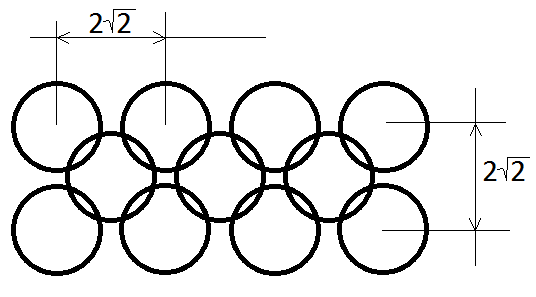
\includegraphics[scale=0.5]{distance_between_particles.png}
\end{center}

Координаты центра данного прямоугольного параллелепипеда можно рассчитать по формулам:

\begin{equation}\label{eq:r_scalar}
    \begin{cases}
        y = \displaystyle\frac{r_b * (K - 1) + 2R}{2},
        \\
        \\
        z = \displaystyle\frac{r_b * (K - 1) + 2R}{2},
        \\
        \\
        x = \displaystyle\frac{r_b * (2 * K - 1) + 2R}{2}.
    \end{cases}
\end{equation}
где $ r_b $ - это расстояние между одинаковыми слоями объёмноцентрированного кристалла, равное $ 2R*\sqrt{2} $, $ K $ - количество частиц в ребре куба по $ Y $ и $ Z $, это число задаётся при новом "посеве" частиц (см. главу "Описание управляющих команд программы").

2. Созданный кристалл копируется несколько раз так, чтобы увеличить кристалл вдвое по трём измерениям ($x$, $y$, $z$), таким образом, делается 7 копий созданного на шаге №1 кристалла, которые располагаются вплотную к первоначальному кристаллу так, чтобы частицы, находящиеся на границах параллелепипедов, касались друг друга.

В результате получается кристалл жёстких сфер в форме прямоугольно параллелепипеда, один угол которого совпадает с началом координат и одна сторона которого в два раза больше двух других сторон.

3. Для частиц, находящихся в кристалле, созданном на шаге №1, случайным образом задаются скорости $ v_x $, $ v_y $ и $ v_z $, при этом скорости остальных частиц в системе задаются так, чтобы суммарный импульс и момент импульса системы были равны нулю.

4. Основываясь на задаваемой плотности системы рассчитываются параметры моделируемого объёма $ A $ и $ L $, а так же коэффициент расширения $ \beta $ (мы рассмотрим подробнее вывод коэффициента расширения системы чуть ниже), на который умножаются все координаты частиц, благодаря чему объёмноцентрированный кристалл жёстких сфер расширяется до размеров моделируемой системы и частицы перестают касаться друг друга. При этом суммарный импульс и момент импульса системы остаются равными нулю, т.к. импульсы одних частиц уравновешены импульсами других частиц, расположенных симметрично относительно центра моделируемой системы.

5. Все частицы копируются ещё раз и их координаты изменяются параллельным переносом вдоль оси $ OX $ так, чтобы в результате частицы заполнили весь объём системы, заданный из расчёта $ L = 4*A $. Скорости частиц не изменяются, поэтому общий импульс и момент импульса системы при этом так же не изменяются. Таким образом размер системы вдоль оси $ OX $ получается в четыре раза больше размера системы вдоль осей $ OY$ и $ OZ $, центры идеальных сфер распределены по всему объёму моделируемой системы так, чтобы частицы не проникали друг в друга и суммарный импульс системы и момент импульса системы были равны нулю.

После проведения "посева" состояние системы сохраняется во временный файл и загружается из него. Во время загрузки сохранённого состояния системы мы рассчитываем ближайшие события для каждой частицы и начинаем расчёт динамики системы. Более подробно это описано в главе "Сохранение и загрузка состояния системы".

\subsection{Расчёт коэффициента расширения системы $ \beta $ }
Рассмотрим подробнее вывод коэффициента расширения системы $ \beta $.

Необходимо описать подробно.

\newpage
\section{Динамика моделируемой системы. События}

Существует два метода расчёта динамики системы многих тел:

1. Итеративный. При этом подходе мы рассчитываем каждое следующее состояние системы, перемещая её во времени на некоторое $ \delta t $. После каждого смещения по времени необходимо рассчитать новые положения и скорости каждого тела в системе. 

2. Событийный. При таком подходе мы рассматриваем динамику системы многих тел как последовательность некоторых событий. Событиями в данном контексте называются моменты времени, в которые происходит изменение уравнений движения частиц в системе.
На каждом шаге мы рассчитываем положение всех частиц в момент времени, когда произойдет следующее событие, изменяющее уравнения движения частиц и сразу же переводим всю систему в этот момент времени. После этого необходимо рассчитать изменение уравнений движения частиц и перейти на следующий шаг, рассчитывая новые положения частиц в момент времени, когда произойдёт следующее событие, меняющее уравнение движения частиц.

$ \\ $

Идеальные сферы в моделируемой системе движутся равномерно и прямолинейно в промежутках времени между столкновениями.

Это означает, что во время перемещения каждой частицы в пространстве значение и направление её скорости не изменяется, и это справедливо для всех частиц.

Благодаря тому, что уравнения движения идеальных сфер изменяются только при наступлении определённых 'событий', мы применяем событийный подход при моделировании динамики моделируемой системы.

\subsection{Типы событий}

В рассматриваемой нами системе могут происходить следующие события:

1. Соударение частицы или её "образа" с идеальной стенкой.

2. Соударение частицы или её "образа" с другой частицей или "образом" другой частицы.

3. Создание "образа" для частицы, находящейся в области, близкой к периодическим граничным условиям.

4. Переход частицы из одной "ячейки" в другую.

5. Замена "образа" частицей - "перерождение" частицы при прохождении через периодические граничные условия.

6. Удаление "образа" частицы.

Необходимо описать подробно.


\subsection{Очередь событий}

Представим, что у нас есть несколько частиц в системе и мы рассчитали времена ближайших событий для каждой частицы. Для начала запишем их в один линейный список:

<Вставить картинку случайно расположенных элементов>

Здесь каждое событие представлено в виде прямоугольника, содержащего информацию о номерах частиц, которые будут участвовать в событии, типе событий и времени $ dt $, через которое эти события произойдут в системе.

Пока состояние системы не изменилось не меняется и список ближайших событий для всех частиц в системе. Как только произойдёт первое из этих событий, состояние системы изменится и мы должны будем обнаружить следующее ближайшее событие для той частицы, чьё событие только что наступило (для удобства будем считать что это частица с индексом $ i $). 

При расчёте следующего ближайшего события для частицы $ i $ может оказаться, что одно из уже записанных в данный список событий для другой частицы $ j $ никогда не произойдёт, например, потому что столкновение двух частиц $ i $ и $ j $ произойдёт раньше, чем ранее рассчитанное событие для частицы $ j $. Тогда нам незачем хранить в памяти событие, которое никогда не произойдёт, и мы можем удалить из этого списка старое событие с участием частицы $ j $ и добавить к этому списку новое событие соударение частиц $ i $ и $ j $.

События других частиц, чьи уравнения движения и времена ближайших событий не изменились после наступления события с частицей $ i $, можно не удалять из списка ближайших событий и не рассчитывать их заново, т.к. они не изменятся.

Так как мы рассчитываем динамику системы на основе событийного подхода, на каждом шаге нам необходимо выбирать из списка всех событий событие с наименьшим временем (чтобы выбрать событие, которое произойдёт в системе раньше других). Поиск такого события в списке событий требует последовательного обращения ко всем элементам этого списка и сравнения времени каждого записанного события со временем других событий в этом же списке.

Чтобы упростить задачу определения следующего события в системе упорядочим список событий по времени наступления событий, в порядке возрастания:

<Вставить картинку упорядоченных линейных элементов>

Тогда ближайшее событие системы всегда будет храниться в первой ячейке нашего списка, и нам не нужно будет проверять все события в этом списке на каждом шаге расчёта динамики системы.

При расчёте следующего ближайшего события для частицы $ i $ необходимо будет вставить новое событие в список событий так, чтобы упорядоченность списка не была нарушена, т.е. необходимо проверить события, уже находящиеся в очереди событий и вставить новое событие в некоторую позицию в данном списке так, чтобы последовательность событий не нарушилась.

Сформулируем правила для 'очереди событий':

1. В очереди событий в каждый момент времени хранится информация о ближайших событиях для всех частиц и 'образов' частиц, если эти 'образы' существуют;

2. В очереди событий хранится информация только о ближайшем событии для каждой частицы и 'образа'. Информация о неактуальных событиях удаляется из очереди событий;

3. Элементы в очереди событий расположены упорядочено, в порядке возрастания времени до наступления события;

4. Для каждой частицы и для каждого существующего в системе образа в очереди событий хранится только одно событие. Это значит, что число событий в очереди событий не может быть больше, чем $ 2N $, где $ N $ - число частиц в системе(здесь мы учитываем, что у каждой частицы может быть только один образ).



\subsection{Бинарное дерево как структура данных}
Бинарное (двоичное) дерево - это структура данных, представляющая собой совокупность элементов и отношений, образующих иерархическую структуру этих элементов.

Если представить бинарное дерево в виде диаграммы, то оно напоминает настоящее перевёрнутое дерево с ветвями:

\begin{center}
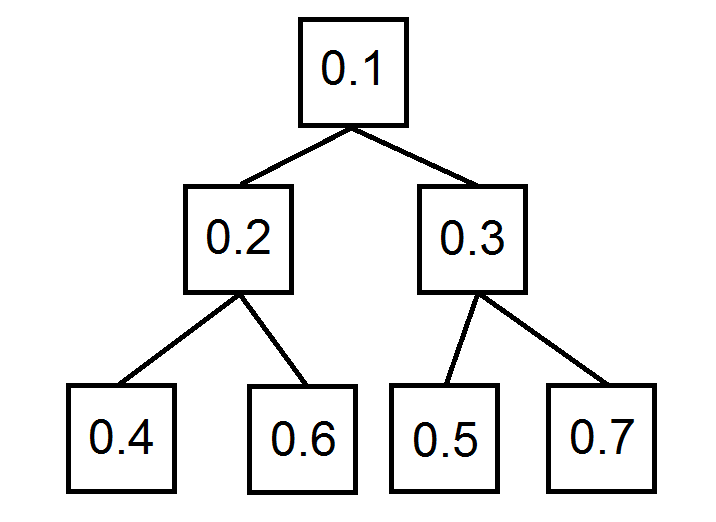
\includegraphics[scale=0.3]{binary_tree_intro.png}
\end{center}

Элементы дерева называются вершинами или узлами дерева. Вершины дерева соединены направленными дугами, которые называются ветвями дерева. Начальная вершина дерева называется корнем дерева, ей соответствует нулевой уровень. Листьями дерева называют вершины, в которые входит одна ветвь и из которых не выходит ни одной ветви.

Вершины, в которые входят ветви, исходящие из одной общей вершины, называются потомками или наследниками этой вершины, а вершина, из которой выходят эти узлы, называется родительским узлом.  Уровень потомка на единицу превосходит уровень его предка. Корень дерева не имеет предка, а листья дерева не имеют потомков.

\subsection{Бинарное дерево для сохранения информации о всех ближайших событиях в системе}

Для сохранения информации о событиях в системе мы будем использовать упорядоченное нестрогое двоичное дерево, обладающее следующими свойствами:

1. Каждый элемент имеет не более двух дочерних элементов;

2. Значение $ dt $ в любой вершине не меньше, чем значения $ dt $ её потомков;

3. Глубина листьев (расстояние до корня) отличается не более чем на 1 слой;

4. Последний слой заполняется слева направо;

5. Если некоторый родительский элемент имеет два дочерних элемента, то левый дочерний элемент имеет значение $ dt_1 $ меньшее, чем значение правого дочернего элемента $ dt_2 $;



\subsection{Добавление элемента в бинарное дерево}
Необходимо описать подробно.
\subsection{Удаление элемента из бинарного дерева}
Необходимо описать подробно.
\subsection{Сравнение алгоритмов на основе бинарного дерева и линейного массива}
Необходимо описать подробно.



\newpage
\section{Собственные времёна частиц и глобальное время системы}
Необходимо описать подробно.

\subsection{Изменение положения частиц в системе}
Необходимо описать подробно.

\subsection{Синхронизация частиц}
Необходимо описать подробно.

\subsection{Поиск ближайшего события для частицы}
Необходимо описать подробно.



\newpage
\section{Сохранение и загрузка состояния системы}
Необходимо описать подробно.

\newpage
\section{Измерение относительной плотности}
Необходимо описать подробно.

\newpage
\section{Получение данных о структуре системы}
Необходимо описать подробно.
\subsection{Профиль плотности}
Необходимо описать подробно.
\subsection{Исследование структуры выделенного слоя частиц. Разрезы}
Необходимо описать подробно.
\newpage
\section{Изменение объёма системы}
Необходимо описать подробно.

\newpage
\section{Измерение давления}
Данная часть алгоритмов и программы ещё не реализовано, необходимо добавить описание того, как мы будем производить измерения данных и описать реализацию алгоритма в программе.

\newpage
\section{Измерение химического потенциала}
Данная часть алгоритмов и программы ещё не реализовано, необходимо добавить описание того, как мы будем производить измерения данных и описать реализацию алгоритма в программе.


\newpage
\section{Описание управляющих команд программы}
Для управления ходом компьютерного эксперимента необходимо использовать управляющие команды, которые должны быть последовательно описаны в текстовом файле $ program.txt $ в директории с запускаемой программой. Программа последовательно считывает управляющие команды и файла $ program.txt $ и так же последовательно выполняет их, выводя информацию о текущей задаче на экран.

Все команды имеют строго определённый синтаксис, опечатки и неправильная последовательность аргументов, пустые строки и некорректные символы в файле описания хода эксперимента могут привести к аварийному завершению программы, сохранению данных в неправильные файлы и даже перезапись уже существующих экспериментальных данных (если в программе эксперимента будет указано, что нам необходимо сохранить некоторые данные в уже существующий файл). Необходимо аккуратно заполнять файл описания эксперимента $ program.txt $ и проверять его содержимое до запуска эксперимента.

Все функции, которые вызываются для выполнения команд, детально описаны отдельно в различных главах данной статьи.

Рассмотрим подробнее каждую управляющую команду, параметры для различных команд и примеры использования.

\subsection{new}
$ new $ - команда, позволяющая запустить процедуру инициализации начального состояния системы (см. главу Посев). 

\uline{Аргументы:}

- Количество частиц в ребре куба объёмноцентрированного кристалла, который будет использоваться во время посева. От числа частиц в ребре этого куба зависит конечное число частиц в моделируемой системе. Например, если число частиц в ребре равно 2, то всего частиц в системе будет 64, если число частиц ребре равно 8, то частиц в системе будет 6976.

- Относительная плотность частиц в системе, которую необходимо задать при инициализации начального состояния. Данная плотность не может быть больше 0.68 (максимальная относительная плотность кристалла с объёмноцентрированной кристаллической решёткой).

\uline{Пример:}

$ new \;\; 8 \;\; 0.4 $

Данная команда создаст новую систему из 6976 частиц, начальная относительная плотность частиц в системе $ \eta $ будет равна 0.4. После инициализации системы так же будут рассчитаны времена ближайших событий для каждой частицы.

После выполнения этой команды мы можем использовать другие управляющие команды, такие, как $ step $, $ compress $, $ profile $ и т.д.


\subsection{save}
Для сохранения состояния системы используется команда $ save $. При сохранении состояния системы в указанный нами текстовый файл будут сохранены число частиц в системе, число "образов" частиц, существующих на данный момент в системе, параметры объёма $ A $ и $ L $ моделируемой системы а так же координаты и скорости каждой частицы и всех существующих на данный момент времени в системе "образов" частиц.

В дальнейшем сохранённое состояние системы можно будет загрузить с помощью команды $ load $.

\uline{Аргументы:}

- Имя текстового файла, в который необходимо сохранить данные о состоянии системы. Если этот файл не существует, он будет создан в директории с программой или по указанному пути, если указать имя файла с полным путём к нему. Если такой файл уже существует, то существующий файл будет перезаписан новыми данными.

\uline{Пример:}

$ save \;\; save\_file\_0.40000\_10000.txt $

Данная команда создаст файл $ save\_file\_0.40000\_10000.txt $ в папке с программой и запишет в этот файл информацию о текущем состоянии системы.

Рекомендуем в имени файла, содержащего информацию о системе, добавлять информацию о текущей плотности системы а так же о количестве соударений, прошедших в систем с момента последнего изменения плотности системы. Это поможет в дальнейшем быстро найти необходимое состояние в системе и вспомнить как именно данное состояние было получено.

\subsection{load}
Для загрузки некоторого ранее сохранённого состояния моделируемой системы из текстового файла используется команда $ load $. Данная команда обнуляет текущее состояние системы, загружает данные о состоянии системы из текстового файла и запускает перерасчёт времён ближайших событий для каждой частицы и каждого "образа" в системе.

Для корректной работы данной команды необходимо существование файла с информацией о некотором состоянии моделируемой системы, синтаксис такого файла строго определён и не должен подвергаться ручному изменению, такие файлы создаются автоматически при сохранении некоторого состояния системы с помощью команды $ save $.

\uline{Аргументы:}

- Имя текстового файла, из которого необходимо загрузить информацию о некотором, сохранённом ранее, состоянии системы. Данный файл должен существовать и быть доступным для чтения запускаемой программой, он должен иметь строго определённую структуру и синтаксис. В случае, если указанный файл не существует, программа будет аварийно завершена.

\uline{Пример:}

$ load \;\; save\_file\_0.40000\_10000.txt $

Данная команда загрузит состояние системы из файла $ save\_file\_0.40000\_10000.txt $ и произведёт расчёт времен ближайших событий для всех частиц и "образов" в системе.

После выполнения этой команды мы можем использовать другие управляющие команды, такие, как $ step $, $ compress $, $ profile $ и т.д.

\subsection{step}
Управляющая команда $ step $ позволяет запустить моделирование динамики системы частиц.

\uline{Аргументы:}

- Количество соударений в системе на одну частицу, в течении которых необходимо рассчитать динамику моделируемой системы. Этот параметр должен быть натуральным числом.

\uline{Пример:}

$ step \;\; 1000 $

Данная команда просчитает динамику системы начиная от последнего состояния системы и до тех пор, пока в системе не произойдёт $ 500*N $ соударений между частицами, где $ N $ - количество частиц в системе. Так как в каждом соударении частиц участвует одновременно две частицы, можно считать что при этом в среднем в системе произошло 1000 соударений для каждой частицы, хотя на самом деле для каждой отдельной частицы число соударений будет разным.

В логику расчёта динамики системы частиц входит множество различных операций, все они подробно описаны в данной статье, а в этой главе мы ограничимся описанием управляющей команды $ step $, которая позволяет управлять продолжительностью моделирования динамики этой системы.

\uline{Примечание:}

Мы можем использовать команду $ step $ несколько раз подряд, при этом состояние системы каждый раз не будет сбрасываться и возвращаться в некоторое исходное состояние, команда $ step $ будет использовать текущее состояние системы как исходное. Например, если мы напишем такой алгоритм:

$ step \;\; 1000 $

$ step \;\; 10000 $

то программа рассчитает сначала динамику системы в течении тысячи соударений на каждую частицу в системе, а затем рассчитает динамику системы в течении ещё десяти тысяч соударений, начиная с того состояния системы, на котором мы остановились после расчёта тысячи соударений в системе.

\subsection{compress}
Управляющая команда $ compress $ позволяет изменять параметры объёма моделируемой системы, за счёт чего изменяется относительная плотность частиц в системе. 

Изменение параметров объёма системы происходит вследствие изменения L (длины системы по оси OX), изменяя длину моделируемой системы мы симулируем движение идеальных стенок, которые ограничивают моделируемую систему в плоскостях $ X = 0 $ и $ X = L $.

Существует три типа изменения плотности системы: $ compress\_left\_wall $ , $ compress\_right\_wall $, $ compress\_both\_walls $, которые симулируют, соответственно, движение только левой стенки, движение только правой стенки и движение одновременно двух стенок.

Все три типа процедур изменения параметров системы действуют по примерно одному и тому же алгоритму, который коротко можно описать так:

1. Найти ближайшую к идеальной стенке частицу и определить расстояние $ \Delta r $ от поверхности сферы, ограничивающей частицу, до идеальной стенки.

2. Сдвинуть стенку на расстояние, меньшее $ \Delta r $ и меньшее некоторой заранее определённой $ \Delta L $. Важно отметить, что при смещении одной или нескольких идеальных стенок в системе перерасчёт позиций "образов" частиц произведён не будет, т.к. мы можем перемещать образы вдоль оси $ OX $ не изменяя при этом момент импульса $ L_x $ моделируемой системы.

3. Рассчитать время ближайших событий для всех частиц и образов. 

5. Рассчитать динамику в системе на протяжении некоторого, заранее заданного, числа соударений на каждую частицу.

6. Если относительная плотность частиц в системе не соответствует указанной пользователем в параметрах плотности, то вернуться на шаг №1.

Рассмотрим каждый тип изменения параметров системы в отдельности.

\subsubsection{$ compress\_left\_wall $}
Управляющая команда $ compress\_left\_wall $ позволяет изменять параметры моделируемой системы, симулируя движение "левой" идеальной стенки (имеется ввиду идеальная стенка $ X = 0 $, данная стенка условно называется левой, т.к. на профиле плотности, где представлены данные о значениях относительной плотности в системе, данная граница системы расположена слева, в начале координат).

При этом сама "левая" идеальная стенка не движется, программа производит смещение всех частиц и образов на определённое $ \Delta L $ в сторону этой стенки вдоль оси $ OX $, после чего уменьшает параметр системы $ L $ на ту же величину $ \Delta L $, в результате чего идеальная стенка, ограничивающая моделируемую нами систему в плоскости $ x = 0 $, становится ближе ко всем частицам в системе на расстояние $ \Delta L $ (или дальше, это зависит о того, хотим ли мы увеличить относительную плотность частиц в системе или хотим уменьшить её). Расстояние между частицами и второй идеальной стенкой, ограничивающей систему в плоскости $ x = L $ не изменяется.

Таким образом мы моделируем изменение координаты "левой" идеальной стенки, приближая её ко всем частицам в системе или отдаляя эту границу от них.

Величина $ \Delta L $, на которую мы изменяем расстояние между частицами и стенкой не может быть больше расстояния между идеальной стенкой и самой ближней к ней частице, а так же ограничивается значением максимально допустимого смещения стенки, задаваемого в качестве аргумента для данной команды.

\uline{Аргументы:}

- Относительная плотность системы, которую необходимо установить в системе с помощью движения идеальной стенки. Указываемая относительная плотность частиц в системе может быть как больше, так и меньше текущей плотности в системе, в зависимости от чего с помощью данной команды можно как сжимать моделируемую систему, уменьшая объём, в котором находятся частицы, так и наоборот, расширять данную системы, отодвигая идеальную стенку от частиц и уменьшая относительную плотность системы.

- Значение максимально допустимого смещения стенки $ \Delta L_{max} $. Если ближайшая к идеальной стенке частица находится на расстоянии, большем $ \Delta L_{max} $, то идеальная стенка может быть смещена только на расстояние $ \Delta L_{max} $.

- Число K1 соударений на частицу, которое необходимо рассчитать после каждого маленького изменения плотности моделируемой системы прежде, чем совершить следующее изменение координат идеальной стенки. Данный параметр позволяет задавать интервал изменения плотности системы, что даёт нам возможность изменять плотность на столько медленно, на сколько  это требуется условиями эксперимента.

- Число K2 шагов сжатия (сдвигов стенки), после которого необходимо провести дополнительный расчёт динамики системы (соударений частиц).

- Число K3 соударений на частицу, которое необходимо рассчитать после каждых K2 шагов сжатия системы.

\uline{Пример:}

$ compress\_left\_wall \;\; 0.503423 \;\; 0.000001 \;\; 10 10 10000 $

Данная команда изменит относительную плотность частиц в системе до значения $ 0.503423 $, при этом максимальное расстояние, на которое будет меняться расстояние между частицами и идеальной стенкой будет не более $ \Delta L_{max} = 0.000001 $ и после каждого небольшого изменения плотности системы будет произведён расчёт динамики движения частиц в системе на протяжении десяти соударений на каждую частицу в этой системе.

\uline{Короткая запись команды:}

Данная команда имеет вариант короткой записи, которая имеет те же аргументы и работает так же, как и полная запись команды:

$ compressl \;\; 0.49 \;\; 0.503423 \;\; 0.000001 \;\; 10 10 10000 $

\subsubsection{$ compress\_right\_wall $}
Управляющая команда $ compress\_right\_wall $ позволяет изменять параметры моделируемой системы, симулируя движение "правой" идеальной стенки (данная стенка условно называется правой, т.к. на профиле плотности, где представлены данные о значениях относительной плотности в системе, данная граница системы расположена справа).

На каждом шаге изменения параметров моделируемой системы программа определяет наименьшее расстояние $ \Delta r $ поверхности частиц в системе до идеальной стенки, ограничивающей моделируемую систему в плоскости $ x = L $ и изменяет координаты этой идеальной стенки на величину, меньшую $ \Delta r $. Если расстояние $ \Delta r $ больше, чем задаваемое пользователем максимально допустимое смещение стенки $ \Delta L_{max} $, то стенка смещается на расстояние $ \Delta L_{max} $.

В результате изменения значения параметра системы L идеальная стенка, ограничивающая моделируемую нами систему в плоскости $ x = L $, становится ближе (или дальше, это зависит о того, хотим ли мы увеличить относительную плотность частиц в системе или хотим уменьшить её) ко всем частицам в системе на расстояние $ \Delta L $, расстояние между частицами и второй идеальной стенкой, ограничивающей систему в плоскости $ x = 0 $ не изменяется.

Таким образом мы моделируем изменение координаты "правой" идеальной стенки, приближая её ко всем частицам в системе или отдаляя эту границу от них.

Величина $ \Delta L $, на которую мы изменяем расстояние между частицами и стенкой не может быть больше расстояния между идеальной стенкой и самой ближней к ней частице, а так же ограничивается значением максимально допустимого смещения стенки, задаваемого в качестве аргумента для данной команды.

\uline{Аргументы:}

- Относительная плотность системы, которую необходимо установить в системе с помощью движения идеальной стенки. Указываемая относительная плотность частиц в системе может быть как больше, так и меньше текущей плотности в системе, в зависимости от чего с помощью данной команды можно как сжимать моделируемую систему, уменьшая объём, в котором находятся частицы, так и наоборот, расширять данную системы, отодвигая идеальную стенку от частиц и уменьшая относительную плотность системы.

- Значение максимально допустимого смещения стенки $ \Delta L_{max} $. Если ближайшая к идеальной стенке частица находится на расстоянии, большем $ \Delta L_{max} $, то идеальная стенка смещается только на расстояние $ \Delta L_{max} $.

- Число K1 соударений на частицу, которое необходимо рассчитать после каждого маленького изменения плотности моделируемой системы прежде, чем совершить следующее изменение координат идеальной стенки. Данный параметр позволяет задавать интервал изменения плотности системы, что даёт нам возможность изменять плотность на столько медленно, на сколько  это требуется условиями эксперимента.

- Число K2 шагов сжатия (сдвигов стенки), после которого необходимо провести дополнительный расчёт динамики системы (соударений частиц).

- Число K3 соударений на частицу, которое необходимо рассчитать после каждых K2 шагов сжатия системы.

\uline{Пример:}

$ compress\_right\_wall \;\; 0.49 \;\; 0.0000001 \;\; 1000 10 10000 $

Данная команда изменит относительную плотность частиц в системе до значения $ 0.49000 $, при этом максимальное расстояние, на которое будет меняться расстояние между частицами и идеальной стенкой, будет не более $ \Delta L_{max} = 0.0000001 $ и после каждого небольшого изменения плотности системы будет произведён расчёт динамики движения частиц в системе на протяжении тысячи соударений на каждую частицу в этой системе.

\uline{Короткая запись команды:}

Данная команда имеет вариант короткой записи, которая имеет те же аргументы и работает так же, как и полная запись команды:

$ compressr \;\; 0.49 \;\; 0.0000001 \;\; 1000 10 10000 $


\subsubsection{$ compress\_both\_walls $}
Данная команда позволяет изменять плотность моделируемой системы, двигая одновременно обе идеальные стенки на одинаковое расстояние. Расстояние, на которое необходимо сдвинуть обе стенки выбирается на основании минимального расстояния частиц до обеих идеальных стенок.

\uline{Аргументы:}

- Относительная плотность системы, которую необходимо установить в системе с помощью движения идеальных стенок. Указываемая относительная плотность частиц в системе может быть как больше, так и меньше текущей плотности в системе, в зависимости от чего с помощью данной команды можно как сжимать моделируемую систему, уменьшая объём, в котором находятся частицы, так и наоборот, расширять данную системы, отодвигая идеальные стенки от частиц и уменьшая относительную плотность системы.

- Значение максимально допустимого смещения стенок $ \Delta L_{max} $. Если ближайшая к идеальной стенке частица находится на расстоянии, большем $ \Delta L_{max} $, то идеальная стенка смещается только на расстояние $ \Delta L_{max} $.

- Число K1 соударений на частицу, которое необходимо рассчитать после каждого маленького изменения плотности моделируемой системы прежде, чем совершить следующее изменение координат идеальных стенок. Данный параметр позволяет задавать интервал изменения плотности системы, что даёт нам возможность изменять плотность на столько медленно, на сколько  это требуется условиями эксперимента.

- Число K2 шагов сжатия (сдвигов стенок), после которого необходимо провести дополнительный расчёт динамики системы (соударений частиц).

- Число K3 соударений на частицу, которое необходимо рассчитать после каждых K2 шагов сжатия системы.

\uline{Пример:}

$ compress\_both\_walls \;\; 0.49 \;\; 0.0000001 \;\; 1000 10 10000 $

Данная команда изменит относительную плотность частиц в системе до значения $ 0.49000 $, при этом максимальное расстояние, на которое будет меняться расстояние между частицами и идеальными стенками, будет не более $ \Delta L_{max} = 0.0000001 $ и после каждого небольшого изменения плотности системы будет произведён расчёт динамики движения частиц в системе на протяжении тысячи соударений на каждую частицу в этой системе.

\uline{Короткая запись команды:}

Данная команда имеет вариант короткой записи, которая имеет те же аргументы и работает так же, как и полная запись команды:

$ compresst \;\; 0.49 \;\; 0.0000001 \;\; 1000 10 10000 $


\subsection{image}

Управляющая команда $ image $ собирает информацию об относительной плотности частиц в системе и сохраняет эту информацию в текстовый файл.

Необходимо описать подробно.


\subsection{profile}

Управляющая команда $ profile $ сохраняет информацию о положениях центров частиц в некотором "слое" системы, что позволяет изучать структуру системы жёстких сфер в некоторой выделенной области моделируемой системы. Информация о положении центров частиц в некотором "слое" системы, ограниченным плоскостями $ x_1 = const $ и $ x_2 = const $, называется "разрезом", т.к. позволяет нам увидеть положение центров частиц, находящихся в данном "слое" в проекции на плоскость $ OYZ $.

Необходимо описать подробно.

\newpage
\section{Глоссарий}

\newpage
\bibliographystyle{utf8gost705u}
\bibliography{./biblio2}


\newpage
\section{Приложения}

\subsection{Блок схемы функций и процедур}

\subsubsection{Функция init(). Контроль эксперимента }

Функция проведения эксперимента по указанному в
текстовом файле описанию.


\begin{center}
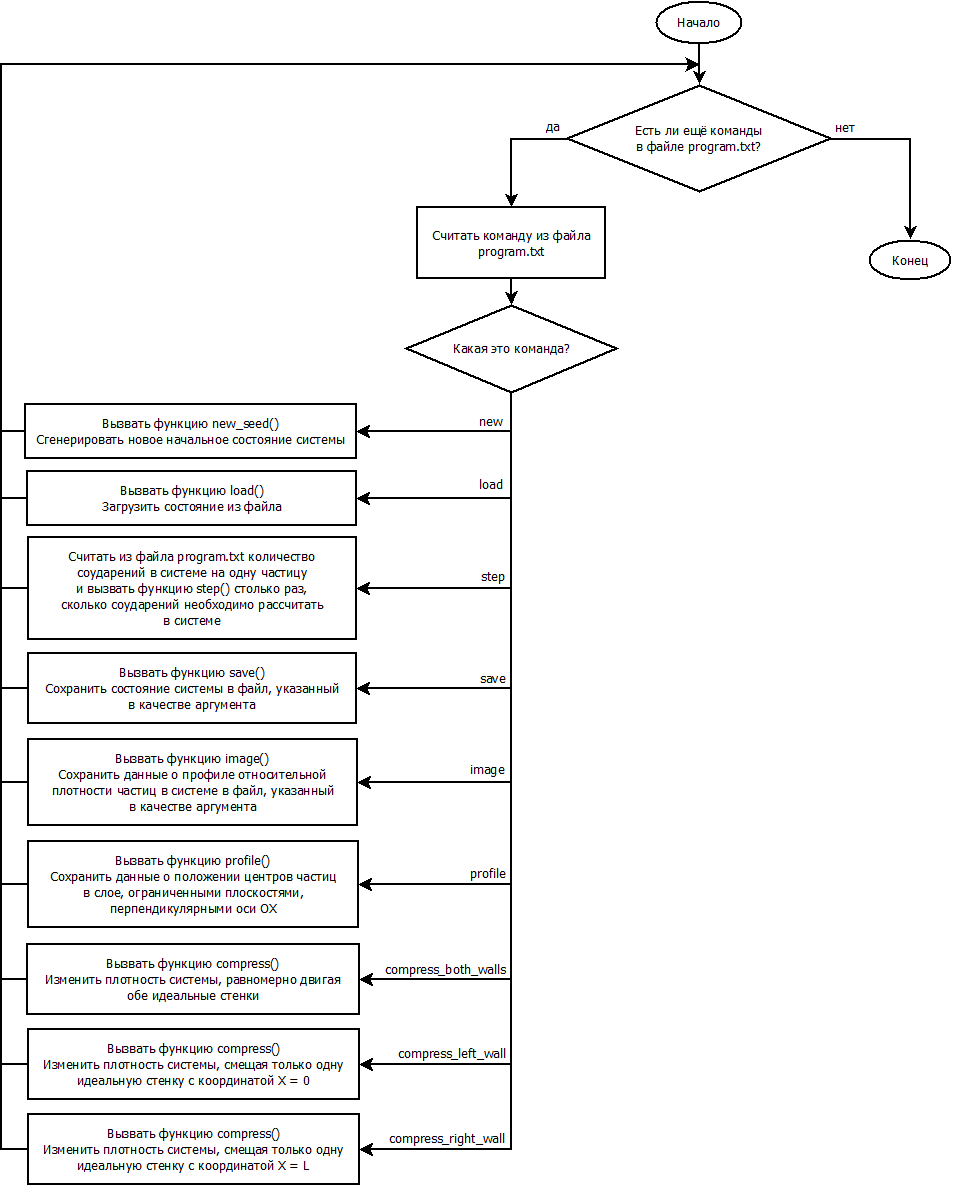
\includegraphics[scale=0.45]{init.png}
\end{center}

\newpage
\subsubsection{Функция step(). Основной цикл программы }

Функция 'шаг', основной цикл программы, производит расчёт динамики системы в течении 1 соударения на каждую частицу, т.е. N/2 столкновений в системе, где N - количество частиц в системе.

\begin{center}
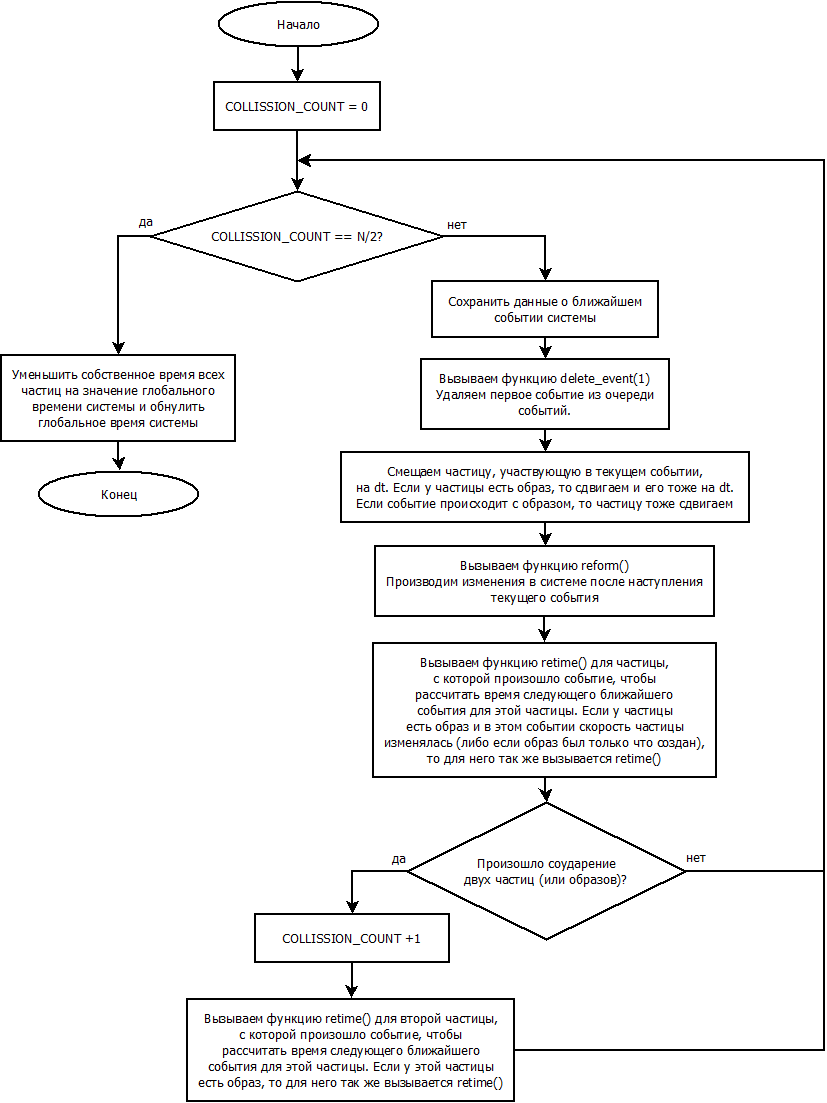
\includegraphics[scale=0.45]{step.png}
\end{center}


\begin{landscape}

\subsection{Исходный код программы с комментариями}
\lstinputlisting{MD2.0.cpp}


\end{landscape}
\subsection{Дополнительные материалы}

\end{document}